% Created 2019-08-25 Sun 14:45
% Intended LaTeX compiler: pdflatex
\documentclass[11pt]{article}
\usepackage[latin1]{inputenc}
\usepackage[T1]{fontenc}
\usepackage{graphicx}
\usepackage{grffile}
\usepackage{longtable}
\usepackage{wrapfig}
\usepackage{rotating}
\usepackage[normalem]{ulem}
\usepackage{amsmath}
\usepackage{textcomp}
\usepackage{amssymb}
\usepackage{capt-of}
\usepackage{hyperref}
\author{Nicol�s Luarte}
\date{\today}
\title{Javiera}
\hypersetup{
 pdfauthor={Nicol�s Luarte},
 pdftitle={Javiera},
 pdfkeywords={},
 pdfsubject={},
 pdfcreator={Emacs 25.2.2 (Org mode 9.2.4)}, 
 pdflang={English}}
\begin{document}

\maketitle
\tableofcontents

\section{Ciclos}
\label{sec:orgcecac95}
\subsection{Ciclo 1}
\label{sec:org0aa11e4}
\begin{center}
\begin{tabular}{lll}
Ejercicio & Protocolo & Bloque\\
\hline
Sentadilla de competencia & x6@8, 10\%, 4x6 & A\\
Sentadilla con pausa (3 ct) & x6@8, 10\%, 2x6 & A\\
Banca de competencia & x6@8, 10\%, 4x7 & A\\
Banca agarre cerrado & x6@8, 10\%, 2x7 & A\\
\hline
Press banca triple pausa & x6@8, 10\%, 3x7 & B\\
Peso muerto de competencia & x3@8, 15\%, 3x4 & B\\
Peso muerto con pausa (3 ct) & x3@8, 15\%, 2x4 & B\\
Peso muerto desde bloques & x3@8, 15\%, 2x5 & B\\
\end{tabular}
\end{center}
\subsection{Ciclo 1 (descarga)}
\label{sec:org7895794}
\begin{center}
\begin{tabular}{lll}
Ejercicio & Protocolo & Bloque\\
\hline
Sentadilla de competencia & x10@8, 10\%, 1x10 & A\\
Estocadas con mancuernas & 3x15 & A\\
Banca de competencia & x10@8, 10\%, 1x10 & A\\
\hline
Peso muerto compentecia & x8@8, 10\%, 1x8 & B\\
Remo con barra & 3x8 & B\\
Curl de biceps & 3x10 & B\\
\end{tabular}
\end{center}
\subsection{Ciclo 2}
\label{sec:org0637e9a}
\begin{center}
\begin{tabular}{lll}
Ejercicio & Protocolo & Bloque\\
\hline
Sentadilla de competencia & x1@8, 20\%, 5x5 & A\\
Sentadilla con pausa (3 ct) & x6@8, 10\%, 2x6 & A\\
Banca de competencia & x1@8, 15\%, 4x7 & A\\
Banca tempo 600 & x1@8, 10\%, 1x4, 10\%, 4x3 & A\\
\hline
Peso muerto de competencia & x1@8, 20\%, 5x5 & B\\
Peso muerto con pausa (3 ct) & x1@8, 10\%, 1x4, 10\%, 1x5 & B\\
Banca de competencia 5sec pausa & x1@8, 10\%, 1x3, 10\%, 4x3 & B\\
Banca sin pausa & x1@8, 20\%, 1x7, 5\%, 1x7, 5\% 1x8 & B\\
\end{tabular}
\end{center}
\section{Comentarios t�cnicos}
\label{sec:org612ce7f}
\subsection{Ciclo 2}
\label{sec:org55365f5}
\subsubsection{Comentario semama del 19/08}
\label{sec:org6fae212}
\begin{enumerate}
\item Squat
\label{sec:orgd7366e1}
\begin{itemize}
\item Falta profundidad
\item Revisa video del d�a lunes y tomar nota de lo que crees que hiciste bien
\item Recuerda baja los pins de seguridad de manera que al bajar no choques con ellos
\item Elongar harto los talones
\item Inflar el estomago contra el cinturon para hacer un brace fuerte
\end{itemize}
\item Banca
\label{sec:org297ec31}
\begin{itemize}
\item Buscar que el press sea diagonal de subida, evitar salir muy vertical
\end{itemize}
\item Peso muerto
\label{sec:org2cfc509}
\begin{itemize}
\item Fijarse que la tomada este simetrica
\item Aun sigues tironeando la barra
\item Recuerda tensar la barra al maximo antes de levantarla
\end{itemize}
\end{enumerate}

\section{Registro de progreso}
\label{sec:org8c2bbab}
\subsection{Ciclo 1}
\label{sec:org056f6d6}
\begin{center}
\label{tab:orgf4620f7}
\begin{tabular}{lrrl}
Ejercicio & RPE & Peso & Fecha\\
\hline
Sentadilla de competencia & 8 & 65 & 08/07/2019\\
Sentadilla con pausa & 8 & 50 & 08/07/2019\\
Banca de competencia & 8 & 32 & 08/07/2019\\
Banca agarre cerrado & 8 & 25 & 08/07/2019\\
Press banca triple pausa & 8 & 25 & 10/07/2019\\
Peso muerto de competencia & 8 & 80 & 10/07/2019\\
Peso muerto con pausa & 8 & 70 & 10/07/2019\\
Peso muerto desde bloques & 8 & 85 & 10/07/2019\\
Sentadilla de competencia & 8 & 70 & 15/07/2019\\
Sentadilla con pausa & 8 & 55 & 15/07/2019\\
Banca de competencia & 8 & 30 & 15/07/2019\\
Banca agarre cerrado & 8 & 25 & 15/07/2019\\
Sentadilla de competencia & 8 & 60 & 23/07/2019\\
Sentadilla con pausa & 8 & 50 & 23/07/2019\\
Banca de competencia & 8 & 35 & 23/07/2019\\
Banca agarre cerrado & 8 & 32 & 23/07/2019\\
Peso muerto de competencia & 8 & 100 & 02/08/2019\\
Peso muerto con pausa & 8 & 90 & 02/08/2019\\
Press banca triple pausa & 8 & 30 & 02/08/2019\\
Sentadilla de competencia & 8 & 60 & 05/08/2019\\
 &  &  & \\
\end{tabular}
\end{center}
\begin{center}
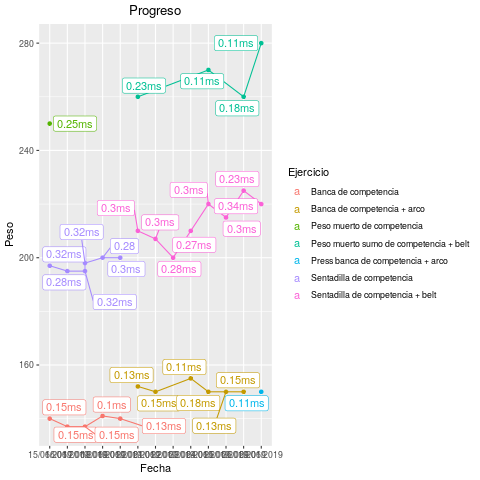
\includegraphics[width=.9\linewidth]{tmp.png}
\end{center}

\subsection{Ciclo 2}
\label{sec:org9b4d1a3}
\begin{center}
\label{tab:orgf38f740}
\begin{tabular}{lrrl}
Ejercicio & RPE & Peso & Fecha\\
\hline
Sentadilla & 8 & 70 & 19/08/2019\\
Banca & 8 & 30 & 19/08/2019\\
Peso muerto & 8 & 105 & 20/08/2019\\
Banca pausada & 8 & 37 & 20/08/2019\\
Sentadilla & 8 & 80 & 22/08/2019\\
Banca & 8 & 40 & 22/08/2019\\
Peso muerto & 8 & 100 & 23/08/2019\\
Banca pausada & 8 & 40 & 23/08/2019\\
\end{tabular}
\end{center}

\begin{center}
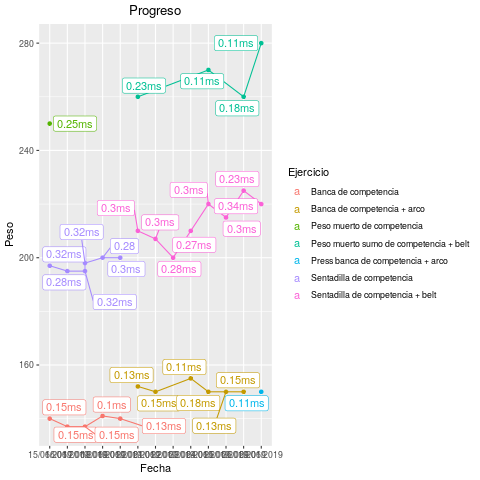
\includegraphics[width=.9\linewidth]{tmp.png}
\end{center}
\end{document}
